
\section{NEFD Methods 1 and 2: deep integration {\color{blue} Nico}}
\label{NEFD_deep}

\subsection{Observations}

\hls is moderately faint source, expected to be below 100~mJy at 1mm and
XX~mJy at 2mm {\bf check values in NIKA1 paper + use SED for predictions in
  NIKA2's bands}. This source was chosen for its flux and its availability during
Run9 for long integration. It has been observed for XX hours in total over three
nights.

As part of the NIKA2 Science Verification that took place in February 2017, we
observed an area of 185~arcmin$^2$, centered on \hls, (a lensed dusty galaxy at
z=5.24 \cite{combes2012}) during about 9~hours. The scans were 8x5~arcmin$^2$,
alternatively oriented in (ra,dec), (dec,ra), (az,el), (el,az).\\


\subsection{Data processing}

The data were decorrelated using the {\tt common-monde-one-block} method
(cf.~\ref{se:cm1blck}), masking a disk of 60~arcsec radius centered \hls.  The
scans have been combined with standard inverse noise weighting. The noise in
each map pixel is derived from the rms of the background corrected by the square
root of the number of observations per pixel (N1). If the noise was perfectly
gaussian, the distribution of the map signal over this noise estimate (far from
the source) would be a normalized gaussian. In practice, this leads to gaussians
that 1.6 and 1.5 larger. We therefore increase our noise estimate (N1) by these
factors to derive our final estimates. Should the extra sources that pop up in
the field contribute to this estimate, they would only make our estimate more
conservative.

\subsection{Detailed methodology and results}

%% \input{hls_1mm.tex}
%% \input{hls_2mm.tex}
%% \input{Pluto.tex}

These data can be used to derive the NEFD in several ways. One is to fit the
evolution of the uncertainty on the flux of the source $\sigma_\phi$ with the
integration time. Another one is to produce jackknife maps with the data and to
measure the uncertainty on the flux in the end, while estimating the time of
integration. Depending on what definition of the time of integration we take, we
might get slightly varying answers, we'll come back to this later one. However,
we must note right now that the assumption that the sensitivity should go like
$1/\sqrt{t}$ needs clarification. This can only be true if scans are co-added
with equal noise weights and are observed under the same conditions of opacity
and elevation. Otherwise, corrections must be taken into account. Indeed, 

\begin{equation}
\sigma = NEFD_0e^{\tau/\sin\delta}\sqrt{t}
\label{eq:sigma_nefd}
\end{equation}

and scans are coadded with inverse variance weighting, so the combined flux is:

\begin{equation}
\phi = \frac{1}{\sum_n 1/\sigma_n^2}\sum_n\frac{\phi_n}{\sigma_n^2}
\end{equation}

whose variance is

\begin{equation}
\sigma^2 = \frac{1}{\sum_n 1/\sigma_n^2}
\end{equation}

which, according to Eq.~(\ref{eq:sigma_nefd}) becomes

\begin{equation}
\sigma^2 = \frac{NEFD_0^2}{\sum_{n}t_n e^{-2\tau_n/\sin\delta_n}}\,.
\label{eq:sigma_tau_w8}
\end{equation}

If the opacity and the elevations are the same for all scans, we recover the
integration like $\sqrt{t}$. In general, if the observing conditions vary, we
must fit the integrated sensitivity vs the effective time $\sum_{n}t_n
e^{-2\tau_n/\sin\delta_n}$ in order to recover an unbiased estimate of
$NEFD_0$. Luckily enough, we have observations of Pluto in very stable
atmospheric conditions and at quasi constant elevation. This will allow us to
check this formalism against more intuitive and direct definitions. We can also
extract from the scans on \hls those that were under stable opacity conditions
and at high and quasi-constant elevation as a confirmation of our final
estimates. The other regimes will help us derive uncertainties our estimates.\\

\begin{figure}[htpb]
\begin{center}
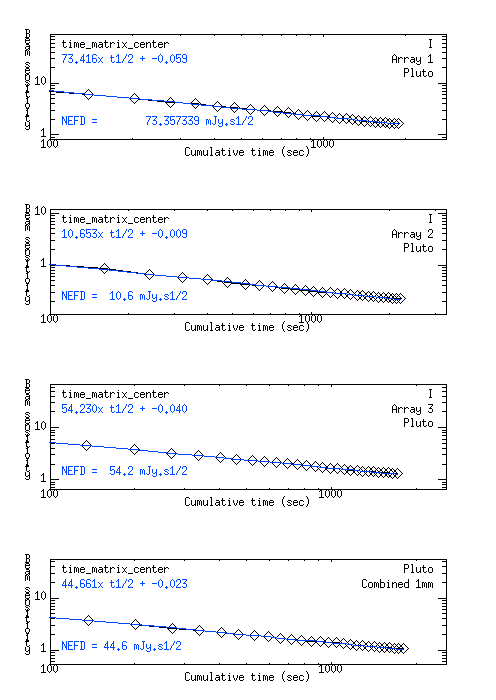
\includegraphics[clip, angle=0, scale=0.4]{Figures/Pluto_8_sigma_vs_time_matrix_center.png}
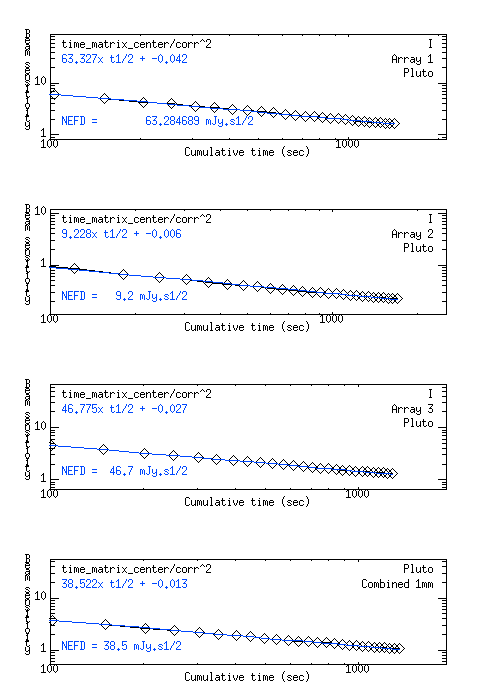
\includegraphics[clip, angle=0, scale=0.4]{Figures/Pluto_8_sigma_vs_time_matrix_center_tau_w8.png}
\caption[Noise decrease with the integration time]{\emph{Left:}$1\,\sigma$ sensitivity vs $t_{int}$ during observations of Pluto, {\bf
  without correction for elevation or opacity}. \emph{Right:} Same fit but this
  time considering the effective time, weighted by opacity and elevation as in Eq.~(\ref{eq:sigma_tau_w8}).}
\label{fig:Pluto_8_sigma_vs_time_matrix_center}
\end{center}
\end{figure}


\begin{figure}[htpb]
\begin{center}
\includegraphics[clip, angle=0, scale=0.4]{Figures/Pluto_5_opacity.eps}
\includegraphics[clip, angle=0, scale=0.4]{Figures/Pluto_5_elevation.eps}
\includegraphics[clip, angle=0, scale=0.4]{Figures/HLS091828_5_opacity.eps}
\includegraphics[clip, angle=0, scale=0.4]{Figures/HLS091828_5_elevation.eps}
\caption[Observing conditions during the noise integration tests]{Opacities and elevations during observations of Pluto and \hls. While
  conditions were stable both in opacity and elevation for Pluto, it was not the
case for \hls.}
\label{fig:pluto_opacities}
\end{center}
\end{figure}

\paragraph{Pluto.} We have 28 scans of Pluto, for a total
integration time of XX at 1mm and XX at
2mm. Fig.~\ref{fig:Pluto_8_sigma_vs_time_matrix_center} shows how the
$1\,\sigma$ sensitivity decreases with $t_{int}$. Considering the small
variations of opacity and elevation during these observations of Pluto
(Fig.~\ref{fig:pluto_opacities}), we can derive an average correction
$exp(-\tau/\sin\delta) = exp(-0.07/\sin(30^\circ)) = 0.87$. This leads to zenith
$NEFD_0^{1mm} = 38.8$ and $NEFD_0^{2mm} = 9.2$\,mJy.s$^{-1/2}$. Using the
jackknife maps and applying the same opacity-elevation correction, one gets
$NEFD_0^{1mm}=38.0$ and $NEFD_0^{2mm}=8.96$.

In light what is discussed in the previous paragraph, if we fit the sensitivity
vs $\sum_{n}t_n e^{-2\tau_n/\sin\delta_n}$, we obtain $NEFD_0^{1mm} = 38.5$ and
$NEFD_0^{2mm}=9.2$. These value are summarized in
tables~\ref{tab:nefd_stable_1mm} and \ref{tab:nefd_stable_2mm}. All these
numbers are obtained with the standard reduction method, a.~k.~a. {\tt
  common\_mode\_one\_block, (CMB)}. If we further subtract a polynomial of order
5 per subscan after this decorrelation (still masking the source), we improve
the results as reported in the tables, while not changing the measured fluxes of
Pluto and HLS (tab.~\ref{tab:fluxes}). We therefore do not change the
calibration with this extra filtering, so the gain in sensitivity does come from
better noise subtraction.

\paragraph{\hls.} While we have an overall
longer integration on \hls, it was acquired during distinct periods, over
varying elevation and different (albeit almost constant by plateau)
opacities (Fig.~\ref{fig:hls_opacities}). Still, performing the same analyses, we obtains the results presented
in tables~\ref{tab:nefd_stable_1mm} and \ref{tab:nefd_stable_2mm}. The values
obtained from the fit vs $1/\sqrt{t}$ are recalled to illustrate the impact of
the opacity-elevation correction on this estimator on \hls\ data. One should
focus on the values derived from the Jackknivfe maps and thoses including the
opacity-elevation correction $1/\sqrt{t_{eff}}$: these values are in very good
agreement when derived from the same reduction method, and in good agreement
between Pluto and \hls.\\

{\bf Conclusion}: while uncertainties on these values should be further
investigated, the good agreement between alternative estimates and at the same
time their differences indicate that they should be valid at about $\pm 1$\,mJy.s$^{1/2}$.
{\bf With these two estimators (fit vs time of integration and
  Jackknife), we find zenith $NEFDs$ below 35 and 9\,mJy.s$^{1/2}$ at 1 and
  2\,mm respectively.} While less intuitive, the more rigourous definition of
the integration time that enters the estimation of the flux, $t_{beam}$, leads to
  slightly different values. It improves by 5\% at 1\,mm, i.e. puts the upper limit at 33.4, but
  degrades the 2\,mm value by the same amount and raise the upper limit to 9.3.

\begin{table}
\begin{tabular}{|l|l|l|l|l|}
\hline
$NEFD_0^{1mm}$~mJy.s$^{1/2}$ & \multicolumn{2}{|c|}{Pluto} & \multicolumn{2}{|c|}{\hls}\\
\hline
Red.~method             & CMB     & CMB+poly5     & CMB & CMB+poly5\\
\hline
$\sim 1/\sqrt{t}$       & 38.8  & 34.3  & 41.7 & 38.2\\
$JK$                    & 35.9  & {\bf 34.7}  & 33.8 & {\bf 33.6} \\
$\sim 1/\sqrt{t_{eff}}$ & 38.5  & {\bf 32.8}  & 37.5 & {\bf 34.4} \\
\hline
\hline
\end{tabular}
\caption[NEFD at 1mm]{Zenith NEFD's in stable elevation and atmospheric conditions on Pluto
  and \hls\ at 1mm.}
\label{tab:nefd_stable_1mm}
\end{table}

\begin{table}
\begin{tabular}{|l|l|l|l|l|}
\hline
$NEFD_0^{2mm}$~mJy.s$^{1/2}$ & \multicolumn{2}{|c|}{Pluto} & \multicolumn{2}{|c|}{\hls}\\
\hline
Red.~method             & CMB     & CMB+poly5     & CMB & CMB+poly5\\
\hline
$\sim 1/\sqrt{t}$       & 9.3 & 8.0 & 9.8  & 8.5\\
$JK$                    & 8.8 & {\bf 7.7} & 8.3  & {\bf 7.6} \\
$\sim 1/\sqrt{t_{eff}}$ & 9.2 & {\bf 8.2} & 9.4  & {\bf 8.2} \\
\hline
\hline
\end{tabular}
\caption[NEFD at 2mm]{Zenith NEFD's in stable elevation and atmospheric conditions on Pluto
  and \hls\ at 2mm.}
\label{tab:nefd_stable_2mm}
\end{table}

\begin{table}
\begin{tabular}{|l|l|l|l|l|}
\hline
Fluxes (mJy) & \multicolumn{2}{|c|}{Pluto} & \multicolumn{2}{|c|}{\hls}\\
\hline
Red.~method  & CMB           & CMB+poly5     & CMB           & CMB+poly5\\
\hline
1\,mm        & $15.0\pm 1.1$ & $13.6\pm 0.9$ & $85.2\pm 0.4$ & $85.4\pm 0.4$\\
2\,mm        & $5.0\pm 0.2$  & $5.0\pm 0.2$  & $14.9\pm 0.1$ & $14.9\pm 0.1$\\
\hline
\hline
\end{tabular}
\caption[Measured fluxes of Pluto and \hls\ with two data reduction methods.]{ The
  extra subtraction of polynomial of order 5 per subscan while masking the
  source does not subtract power to the source, hence the derived sensitivities
  with this methods do not need to be recalibrated.}
\label{tab:fluxes}
\end{table}

%% Tab.~\ref{tab:nefd}. Fig.~\ref{fig:nefd_vs_t} shows the decrease of the
%% uncertainty on the measured flux at the center of the map as a function of
%% time. We either fit a power law or fix the power law to -0.5 and fit only the
%% amplitude. Uncertainties on these values have been estimated via a bootstrap
%% method: we randomize the scans and derive the standard deviation of the average
%% of $n$ scans for any $n$ between 1 and the total number of scans. This gives us
%% an estimate of the uncertainty on $\sigma_\phi$ for a time of integration
%% corresponding to $n$ scans. Strictly speaking, all the scans do not have the
%% exact same duration, but the difference is negligible here.

%% \begin{table}
%% \begin{tabular}{|l|l|l|l|l|}
%% \hline
%% Array & Free power law & Fixed power law $t^{-0.5}$ & Jackknife & Instrument \\
%% \hline
%% A1       & $47.9$ mJy.s$^{-0.54}$ & $37.9$ mJy.s$^{1/2}$ & 35.6 mJy.s$^{1/2}$ & $33.3$ (5) mJy.s$^{1/2}$\\
%% A2       & $5.2$  mJy.s$^{-0.51}$ & $4.8$  mJy.s$^{1/2}$ & 5.7  mJy.s$^{1/2}$ & $5.8$  (5) mJy.s$^{1/2}$\\
%% A3       & $38.9$ mJy.s$^{-0.54}$ & $30.6$ mJy.s$^{1/2}$ & 30.4 mJy.s$^{1/2}$ & $28.4$ (4) mJy.s$^{1/2}$\\
%% A1 \& A3 & $28.5$ mJy.s$^{-0.53}$ & $23.6$ mJy.s$^{1/2}$ & 22.4 mJy.s$^{1/2}$ & $21.1$ (3) mJy.s$^{1/2}$\\
%% \hline
%% \end{tabular}
%% \label{tab:nefd}
%% \caption{Noise integration with observation time and associated derivations of
%%   the NEFD. These values do not account for the extra {\color{red} \bf XXXX \%}
%%   uncertainty on absolute calibration.}
%% \end{table}
%       33.325263       5.2024647
%       28.397230       4.5723151
%       21.143376       4.1538804
%       5.7628233       3.3094792


